	%-=-=-=-=-=-=-=-=-=-=-=-=-=-=-=-=-=-=-=-=-=-=-=-=
%
%        LOADING DOCUMENT
%
%-=-=-=-=-=-=-=-=-=-=-=-=-=-=-=-=-=-=-=-=-=-=-=-=

\documentclass[newPxFont,pagenumber]{beamer}
\usetheme{sthlm}
%\usecolortheme{sthlmv42}

%-=-=-=-=-=-=-=-=-=-=-=-=-=-=-=-=-=-=-=-=-=-=-=-=
%        LOADING PACKAGES
%-=-=-=-=-=-=-=-=-=-=-=-=-=-=-=-=-=-=-=-=-=-=-=-=
\usepackage[utf8]{inputenc}
\usepackage[frenchb]{babel}
\usepackage[normalem]{ulem}
\usepackage{caption}
\captionsetup{font=scriptsize}
%\usepackage[font=footnotesize]{subcaption}
% in preamble
\usepackage{chronology}
\usepackage{pgf}
\usepackage{tikz}
\usetikzlibrary{arrows,automata}

\usepackage{nameref}
\makeatletter
\newcommand*{\currentname}{\@currentlabelname}
\makeatother

\graphicspath{ {fig/} }

\usepackage[linesnumbered,ruled,vlined]{algorithm2e}
% add page number
%\usepackage[defaultsans]{cantarell}

\newcommand{\p}{\mathbb{P}}

\setbeamerfont{title}{series=\upshape}
\setbeamertemplate{footline}{\hfill\footnotesize\insertframenumber\hskip3pt\null\vskip3pt}

\newcommand{\argmax}{\mathop{\mathrm{argmax}}\limits}
\renewcommand{\max}{\mathop{\mathrm{max}}\limits}

\renewcommand{\event}[3][e]{%
  \pgfmathsetlength\xstop{(#2-\theyearstart)*\unit}%
  \ifx #1e%
    \draw[fill=black,draw=none,opacity=0.5]%
      (\xstop, 0) circle (.2\unit)%
      node[opacity=1,rotate=45,right=.2\unit] {#3};%
  \else%
    \pgfmathsetlength\xstart{(#1-\theyearstart)*\unit}%
    \draw[fill=black,draw=none,opacity=0.5,rounded corners=.1\unit]%
      (\xstart,-.1\unit) rectangle%
      node[opacity=1,rotate=45,right=.2\unit] {#3} (\xstop,.1\unit);%
  \fi}%

\addto\captionsfrench{%
\renewcommand{\figurename}{\scriptsize {\scshape Figure}}
\renewcommand{\tablename}{\scriptsize {\scshape Table}}
}

%-=-=-=-=-=-=-=-=-=-=-=-=-=-=-=-=-=-=-=-=-=-=-=-=
%        BEAMER OPTIONS
%-=-=-=-=-=-=-=-=-=-=-=-=-=-=-=-=-=-=-=-=-=-=-=-=

%\setbeameroption{show notes}

%-=-=-=-=-=-=-=-=-=-=-=-=-=-=-=-=-=-=-=-=-=-=-=-=
%
%	PRESENTATION INFORMATION
%
%-=-=-=-=-=-=-=-=-=-=-=-=-=-=-=-=-=-=-=-=-=-=-=-=

\title{\normalsize Analyse Sémantique d'un Corpus Exhaustif de Décisions Jurisprudentielles pour l'Élaboration d'un Modèle Prédictif du Risque Judiciaire}
\subtitle{\small Séminaire e-juris
%\includegraphics[width=0.15\paperwidth]{ProfitLossRiskDecisionOutcomeLg.png}
}
%\date{\small{\jobname}}
%\date{\today}
\date{\scriptsize 24 mars 2017}
\author{\textbf{TAGNY NGOMPE Gildas\textsuperscript{\ref{lgi2p},\ref{chrome}}}, Sébastien Harispe\textsuperscript{\ref{lgi2p}}, Jacky Montmain\textsuperscript{\ref{lgi2p}}, Stéphane Mussard\textsuperscript{\ref{chrome}}, Guillaume Zambrano\textsuperscript{\ref{chrome}}}
%\institute{\small\textbf{Directeur}: Stéphane Mussard, Pr. (CHROME, Univ. Nîmes)  \\ \textbf{Co-directeur}: Jacky Montmain, Pr. (LGI2P, Ecole des Mines d'alès) \\ \textbf{Encadrants}: Guillaume Zambrano, Sébastien Harispe}
\institute{%\scriptsize  
\begin{enumerate}
\item LGI2P (École des mines d'Alès) \label{lgi2p}
\item CHROME EA 7352 (Université de Nîmes) \label{chrome}
\end{enumerate}
}

\hypersetup{
pdfauthor = {\author{}: tagnyngompe@gmail.com},
pdfsubject = {},
pdfkeywords = {},
pdfmoddate= {D:\pdfdate},
pdfcreator = {}
}

\begin{document}
\nocite{}

%-=-=-=-=-=-=-=-=-=-=-=-=-=-=-=-=-=-=-=-=-=-=-=-=
%
%	Section: Classification des décisions par utilisation d’une approche semi-supervisée 
%
%-=-=-=-=-=-=-=-=-=-=-=-=-=-=-=-=-=-=-=-=-=-=-=-=
\section{Extraction d'informations sur les demandes}

\begin{frame}{Origine: Extraction des informations sur les demandes}
\begin{block}{Informations pertinentes à extraire}
\begin{itemize}
\item \textbf{Position de la partie}: Intimé
\item \textbf{Catégorie de demande}: Dommages-intérêts pour procédure abusive
\begin{itemize}
\item \textbf{Objet}: Dommages-intérêts
\item \textbf{Fondement}: Articles 1382 code civil et 32-1 code de procédure civile
\end{itemize}
\item \textbf{Quantum demandé}: 20 000 euros
\item \textbf{Résultat} : Rejet
\item \textbf{Quantum accordé} : 0 euros
\end{itemize}
\end{block}
\end{frame}
\begin{frame}{Difficultés}

Expressions implicites, par  \textcolor{orange}{référence}, par \textcolor{blue}{agrégation}, ...

\begin{exampleblock}{Expression de demande}
La société A. conclut à la confirmation du jugement entrepris sauf à
former appel incident sur la disposition du jugement l'ayant déboutée de sa
demande de \textbf{dommages intérêts pour abus de procédure} et elle demande à la cour de
condamner l'appelante à lui payer la somme de \textbf{20 000 euros} à titre de dommages
intérêts ...

%- \textbf{la} condamner à payer une somme de \textbf{283 589 euros} à titre de {\bf dommages et intérêts pour concurrence déloyale},

...
\end{exampleblock}

\begin{exampleblock}{Expression de resultat}
La cour, ... 

Confirme \textcolor{orange}{la décision entreprise} en \textcolor{blue}{toutes ses dispositions},
\end{exampleblock}
\end{frame}


\begin{frame}{Conditions d'évaluation de la catégorisation des décisions}

\begin{itemize}
\item Représentation vectorielle: {\small \[ poids(w*, t) = poids_{local}(w*, t) * poids_{global}(w*) * facteur_{normalisation}\]}
\item Évaluation de différentes configurations:
\begin{itemize}
\item dimensions des vecteurs : 10, ..., 250, ...
\item méthodes de sélection de termes discriminants (p. \ref{notations} \& \ref{featuresSelectors}): $\chi^2, \Delta_{DF}, Marascuilo, NGL, GSS $  ...
\item méthodes de classification: SVM, arbre de décision, KNN, naïf bayésien (avec Wek)
\item méthodes de pondération locale (p. \ref{localWeights}) : TF, LogTF, ATF, TP
\end{itemize}
\item environ 2000 cas inconnus, 
\item dommages-intérêts pour abus de procédure : entrainement 152 positifs, test 39 positifs + 157 négatifs
\item prestation compensatoire : entrainement 100 positifs, test 100 positifs + 100 négatifs
\item ...
\end{itemize}
\end{frame}

\begin{frame}{Sélection des caractéristiques d'une catégorie de décisions}
\label{notations}
\scriptsize 
\textbf{Notations (Pour le corpus d'entrainement)} \\
$w$ : un terme \\
$t$: un texte \\
$L_w$ : longueur de $w$ (nommbre de mots) \\
$c$ : la classe cible ou positive (catégorie de demande)\\
$\overline{c}$ : la classe complémentaire ou négative (inconnue) \\
$N_{c}$ et $N_{\overline{c}}$ : resp. nombre de textes de $c$ et de $\overline{c}$\\
$N_{w,c}$ : nombre de textes de $c$ contenant $w$ \\
$N$ : nombre total de textes dans le corpus ($N = N_{c} + N_{\overline{c}}$)\\
$DF_c$ : proportion de textes du corpus appartenant à $c$ ($\p(c)$ : probabilité qu'un texte pris au hasard soit de la classe $c$ )\\
%$TF_{w \vert c}$ : fréquence d'observations $w$ dans $c$ (en prenant un terme au hasard parmi les (occurences de) termes de $c$) \\
$DF_w$: proportion de documents du corpus contenant $w$ ("Document frequency")\\
$DF_{w \vert c}$ : proportion de documents de $c$ contenant $w$ \\
$DF_{c \vert w}$ : proportion de documents contenant $w$ qui appartiennent à $c$ ($\p(c \vert w)$=)\\
$Occ_{w,t}$: nombre d'occurrences de $w$ dans $t$ \\
$Occ_t$: somme des nombres d'occurrences des termes dans $t$ \\
$TF_{w,t}$: fréquence d'observation de $w$ dans le texte $t$ \\
$SI_{w}$ : score d'importance de $w$ pour $c$

\end{frame}

\begin{frame}{Sélection des caractéristiques d'une catégorie de décisions}
\label{featuresSelectors}
\scriptsize 

\[\Delta_{DF}(w,c) = DF_{w,c} - DF_{w,\overline{c}}\]

\[\chi^2(w,c) = \frac{N ((N_{w,c} N_{\overline{w},\overline{c}}) - (N_{w,\overline{c}} N_{\overline{w},c}))^2}{N_w N_{\overline{w}} N_c N_{\overline{c}}}\]

\[ngl(w,c) = \frac{\sqrt{N} ((N_{w,c} N_{\overline{w},\overline{c}}) - (N_{w,\overline{c}} N_{\overline{w},c}))}{\sqrt{N_w N_{\overline{w}} N_c N_{\overline{c}}}}\]

\[gss(w,c) = (N_{w,c} N_{\overline{w},\overline{c}}) -  (N_{w,\overline{c}} N_{\overline{w},c})\]


Marascuilo:
\[M(w,c) = \frac{(N_{w,c} - N_{w}N_c/N)^2 + (N_{w,\overline{c}} - N_{w}N_{\overline{c}}/N)^2 + (N_{\overline{w},c} - N_{c}N_{\overline{w}}/N)^2 + (N_{\overline{w},\overline{c}} - N_{\overline{w}}N_{\overline{c}}/N)^2 }{N}\]

\end{frame}

\begin{frame}{Sélection des caractéristiques d'une catégorie de décisions}
\begin{exampleblock}{Dommages-interets pour abus de procedure}
\small
\begin{tabular}{l|c}
\textbf{Terme (n-gram)} & \textbf{Poids global (NGL)}  \\ \hline
\midrule
procédure abusive & 15.710 \\ \hline
pour procédure abusive & 15.007 \\ \hline
pour procédure & 14.890 \\ \hline
abusive & 13.721 \\ \hline
intérêts pour procédure & 10.306 \\ \hline
abus & 10.288 \\ \hline
intérêts pour procédure abusive & 9.984 \\ \hline
32-1 & 9.534\\ \hline
%et intérêts pour procédure & 9.341 \\ \hline
%dommages et intérêts pour procédure & 9.341 \\ \hline
... & ...
\end{tabular}
\end{exampleblock}
$ngl(w,c) = \frac{\sqrt{N} ((N_{w,c} N_{\overline{w},\overline{c}}) - (N_{w,\overline{c}} N_{\overline{w},c}))}{\sqrt{N_w N_{\overline{w}} N_c N_{\overline{c}}}}$ %\cite{ng1997ngl}
\end{frame}

%\begin{frame}{Méthode de pondération locale}
%\label{localWeights}
%\scriptsize 
%
%\begin{table}[!htb]
%\centering
%\begin{tabular}{|p{0.4\textwidth} p{0.4\textwidth}|}
%\hline
%\textbf{Méthode} & \textbf{Formule}  \\ \hline
% &  \\
%Fréquence de $w*$  & $TF_{w*,t} = \frac{Occ_{w*,t}}{\sum\limits_{w_i \in W} Occ_{w_i,t}}$ \\ \hline
% &  \\ 
%Présence de $w*$  & $TP_{w*,t} = \left\lbrace \begin{array}{cl}
%1 & \text{si }TF_{w*,t} > 0 \\
%0 & sinon
%\end{array} \right.$ \\ \hline
% &  \\ 
%Fréquence augmentée de $w*$ & $ATF_{w*,t} = k + (1-k) \frac{TF_{w*,t}}{\max\limits_{w_i \in W} TF_{w_i,t}}$  \\ \hline
% &  \\ 
%Logarithme de la fréquence de $w*$ & $LogTF_{w*,t} = \log{(TF_{w*,t}+1)}$  \\ \hline
%\end{tabular}
%\caption{Méthodes de pondération locale} \label{PoidsLocal}
%\end{table}
%\end{frame}

\begin{frame}{Mesures d'évaluation}
\scriptsize
\[ Precision_C = \frac{\text{\# de décisions test classées par le modèle dans C effectivement de C}}{\text{\# de décisions test effectivement dans C }} \]
\[ Rappel_C = \frac{\text{\# de décisions test de C correctement classées par le modèle dans C }}{\text{\# de décisions test effectivement dans C }} \]
\[ F1_C = 2 \times \frac{Precision_C \times Rappel_C }{Precision_C + Rappel_C} \]

avec $C$ = une classe de décision

\end{frame}

\begin{frame}{Résultats de la classification des décisions}
%\scriptsize
%Est-ce l'effet de la méthode de :
%\begin{itemize}
%\item constitution des exemples d'apprentissage/test
%\item sélection de caractéristiques
%\end{itemize}
\begin{figure}
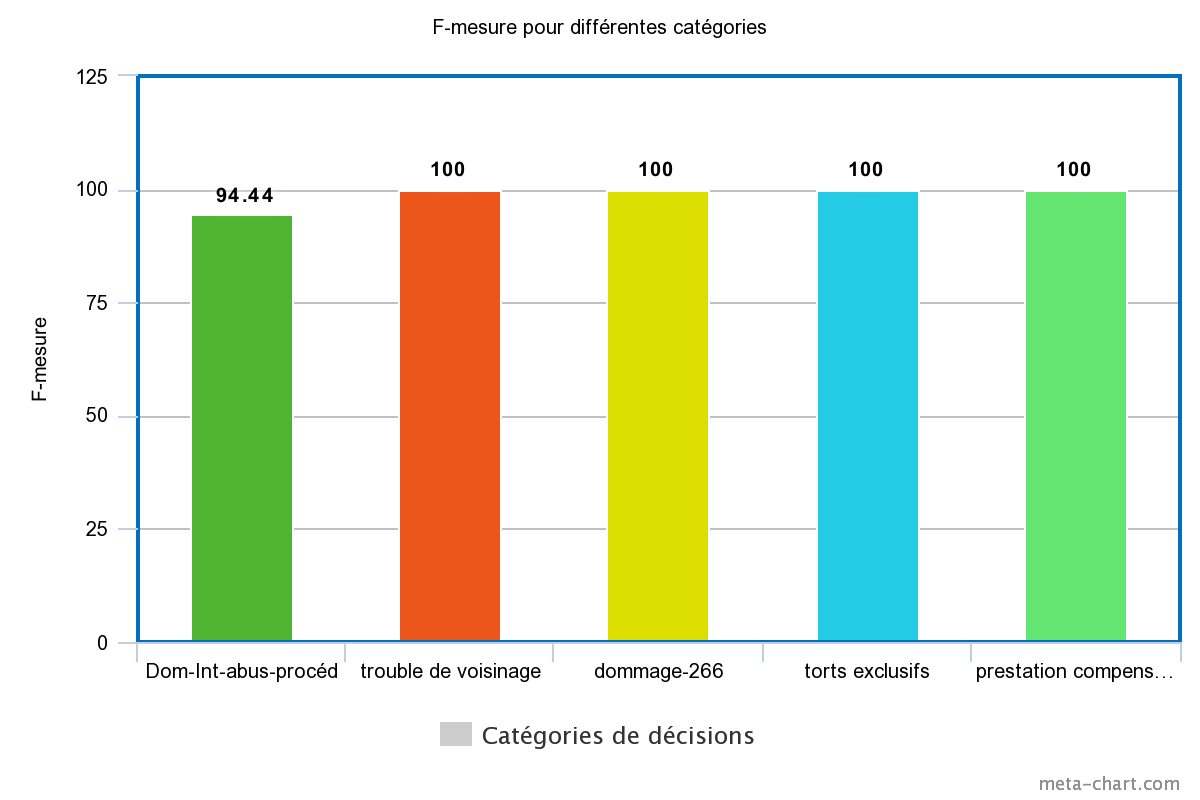
\includegraphics[width=0.9\textwidth]{f-mesure-classif.png}
\caption{Performance actuelles de classification}
\end{figure}
\end{frame}


\begin{frame}{Interprétation des résultats pour une catégorie}
Tentative par classification des décisions
\begin{figure}
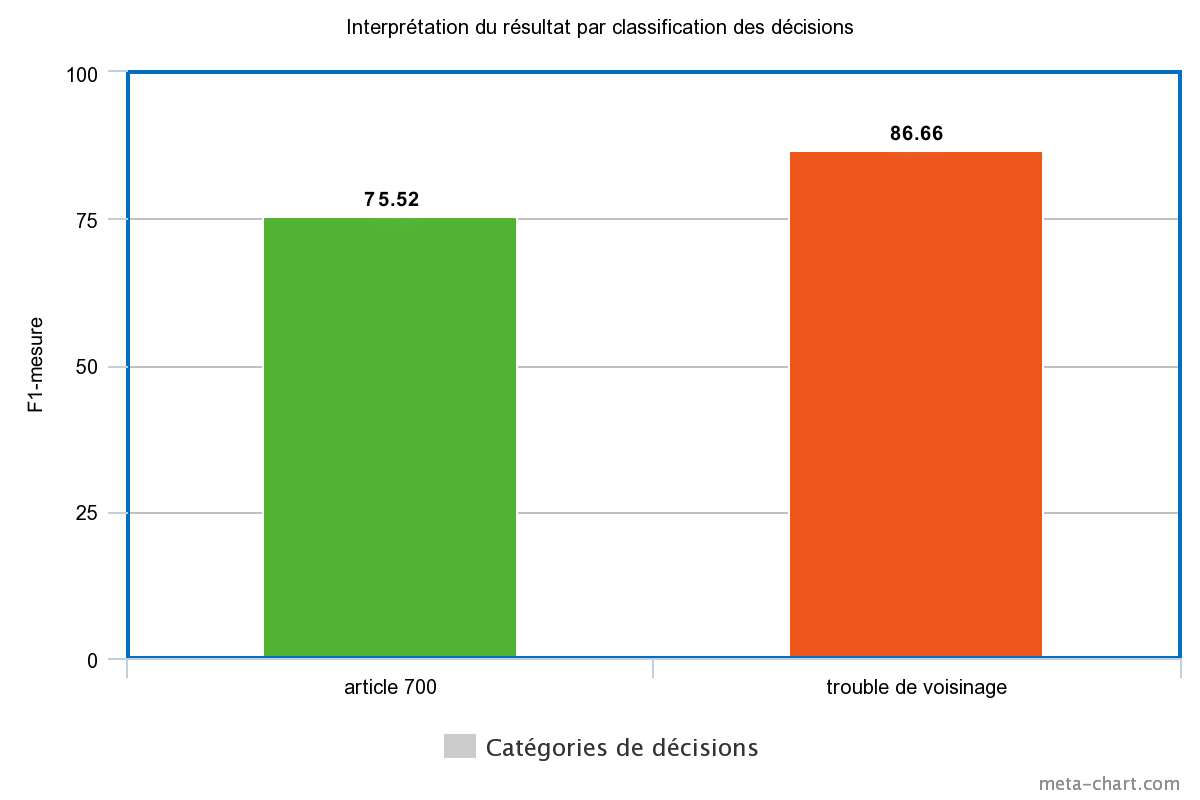
\includegraphics[width=0.8\textwidth]{classifResultat.png}
\caption{Résultats des meilleures configurations (taille des vecteurs, poids global, poids local, modèle de classifieur)}
\end{figure}
\end{frame}

\end{document}
